\chapter{Linear System Solution Methods} \label{LS} 

This chapter presents the popular approaches used for solving linear systems, namely, 
direct and iterative solver techniques.  There are mainly two classes of linear systems-- sparse and dense. The linear systems with majority of the matrix elements as zero are known as sparse linear systems. The systems with most of the elements as non-zero are referred to as dense systems. A common approach of storing sparse matrices involves storing only the non-zero elements, along with their row and column indexes. For dense systems, all elements need to be
stored, including the zero elements. Problems from various application evolve continuously in time, and can be well represented by large sparse linear systems. Therefore, in this dissertation the main focus is on sparse linear systems.

This chapter presents the two main categories of solvers: direct and iterative, and describes some popular solver techniques which include (1) single-method solver schemes, where only one solver is applied for solving the system, (2) multi-method solver schemes, where more than one solvers are used during different solve stages. 

\section{Motivation}
The solution of large sparse linear systems of the form $Ax = b$, where $A = [a_{ij} ]$ is an $n \times n$ matrix and $b$ is a given right-hand-side vector, is an elementary problem in scientific computing. Advancements in domains such as multi-physics, aerodynamics and others, where the problems can be formulated as partial differential equations, rely heavily on the efficient solution of the linear systems. Frequently, the total time in such formulations is predominated by the time taken to solve the linear systems.

\begin{figure}
\begin{center}
 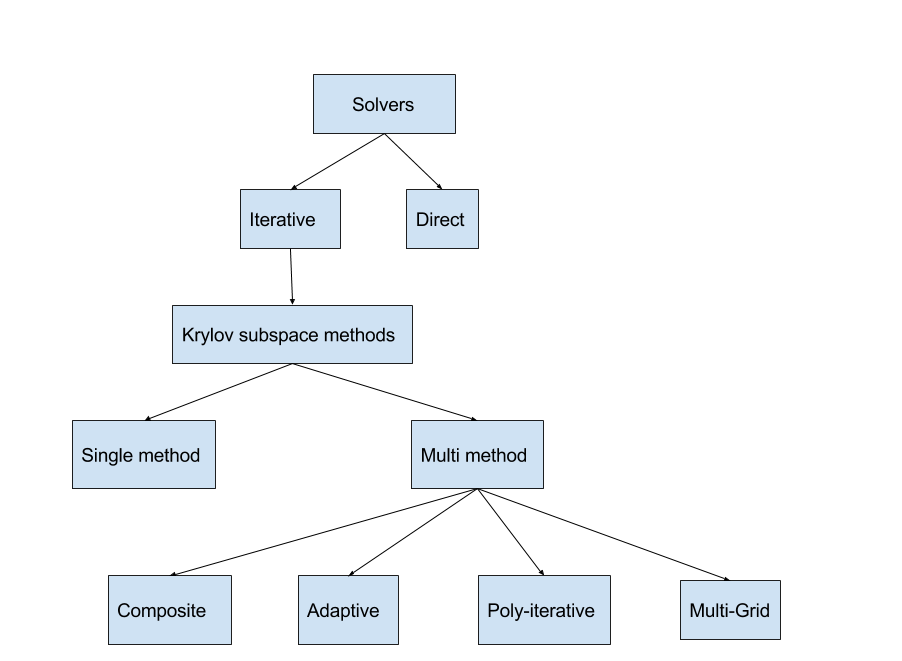
\includegraphics[width=0.95\linewidth]{figures/solver.png}
\end{center}
 \caption{Solver hierarchy showing the different solving strategies.}
 \label{fig:solver}
\end{figure}

The general strategy of solving a sparse linear system of the form $Ax = b$, 
involves transforming the system, $A$ into a similar system which has the same solution, $x$ 
and that is easier to solve. The process of transforming the system into a new system with a reduced condition number, is referred to as preconditioning~\cite{misc3}. Preconditioning is achieved by combining a solver method with a preconditioner. One such transformation 
is pre-multiplying the linear system ($A$) with a non-singular matrix, denoted by $P$. In other words, multiplying 
the left-hand side and the right-hand side with a non-singular matrix. The preconditioning process leaves the solution of the system unaffected. 

There are two popular techniques of solving the systems, namely, direct and iterative solving strategies. Direct solvers have high numerical accuracy and work even for sparse matrices with irregular patterns. Iterative solvers use an initial guess to get an approximation of the solution. For a given approximation solution $x_{k-1}$, the solution, $x_{k}$, at the next iteration is expected to be better. Iterative solvers keep updating the solution until it gets close enough to the actual solution. Figure~\ref{fig:solver} shows the hierarchy of the sparse linear solvers, some of which are discussed in detail in the later sections.


\section{Direct Solvers} \label{DirectSolvers}
For linear systems $Ax=b$, where $A$ is the coefficient matrix, $x$ is the unknown vector and $b$ is the right hand side vector, direct solvers ~\cite{direct1, direct2} provide an exact solution, $x = A^{-1}b$ for the linear system and are more robust than the second category of solvers-- iterative solvers. Direct solvers are preferable for small matrices and in cases where an exact solution is required. However, they are less desirable for very large matrices because of their high costs. This is because the memory requirement for direct solvers can be huge, as direct solvers need the entire matrix to be in memory. For the work presented throughout this dissertation, we focus on sparse matrices. For sparse matrices, most of the elements are zero, therefore storing the entire matrix can be avoided and is rather expensive. This section describes some of the most commonly used direct solvers.


\subsection{LU Factorization Method}
One of the common techniques to solve large linear systems is based on factorization of the matrix $A$ into triangular factors. The transformation of a general system into triangular systems decomposes the original problem into smaller factors, without changing the solution of the system. Converting the original system $Ax = b$ into an equivalent triangular form can be achieved by many ways, such as Gaussian elimination.

For a $n \times n$ matrix $A$, LU factorization factors the original matrix $A$ into the product of the lower triangle of the matrix, represented by $L$ and the upper triangle of the matrix, represented by $U$. In other words, the factorization can be shown by the equation: $A = LU$, where $A$ is the original matrix, $L$ is the lower triangle and $U$ is the upper triangle. A $n \times n$ square matrix $L=(l_{ij})$ is said to be the lower triangular if $l_{ij} = 0$ for $i$ \textless $j$, such that all elements above the diagonal are zero. An $n \times n$ square matrix $U = (u_{ij})$ is considered to be the upper triangle if $u_{ij}$ = 0 for $i$ \textgreater $j$ such that all elements below the diagonal are zero. The factorization can be represented by the following equation: 


\begin{gather} %
\begin{pmatrix}
A_{11} & A_{12} & A_{13} \\
A_{21} & A_{22} & A_{23} \\
A_{31} & A_{32} & A_{33} \\
\end{pmatrix} 
=
\begin{pmatrix}
L_{11} & &  \\
L_{21} & L_{22} &  \\
L_{31} & L_{32} & L_{33} \\
\end{pmatrix}
.
\begin{pmatrix}
U_{11} & U_{12} & U_{13} \\
& U_{22} & U_{23} \\
&  & U_{33} \\
\end{pmatrix}
\end{gather}


The $LU$ factorization of $A = (a_{ij})$ can be given as the product of the matrices $L$ and $U$ as shown in the above equation. The matrix $L$ should have only ones on the diagonal. The matrices $L$ and $U$ are obtained by applying various row operations to make all the elements below the diagonal and all the elements above the diagonal as zero respectively. The next step involves applying forward and backward substitution to get the solution and the total solution time is dominated by the decomposition of $A$ into matrices $L$ and $U$. Forward and backward substitution are shown below.

Forward substitution for lower triangular system can be given as follows: \\
\begin{center}
$x_{1} = b_{1}/a_{11}$ \\
$x_{i} = \lbrack b_{i} - \sum_{j=1}^{i-1} a_{ij} x_{u} \rbrack / a_{ii}$, where $i = 2, \ldots, n$

Backward substitution for upper triangular system can be given as follows:
\\
$x_{n} = b_{n}/a_{nn}$ \\
$x_{i} = \lbrack b_{i} - \sum_{j=i+1}^{n} a_{ij} x_{j} \rbrack / a_{ii}$, where $i = n-1, \ldots, 1$
\end{center}


\subsection{Cholesky Method}
The Cholesky method is a popular direct method for symmetric positive definite matrices, and the factorization can be shown by the equation:
$A = LL^{T}$, where $L$ is a lower triangle matrix with positive entries on its diagonal. The factorization is shown in the set of equations shown below:

\begin {align*}
 A &= 
    \begin{bmatrix}
     a_{11}       & a_{21} & a_{31} \\
     a_{21}       & a_{22} & a_{32} \\
     a_{31}       & a_{32} & a_{33} 
    \end{bmatrix} \\
&= 
    \begin{bmatrix}
     l_{11}       & 0 & 0 \\
     l_{21}       & l_{22} & 0 \\
     l_{31}       & l_{32} & l_{33} 
    \end{bmatrix}
       . 
    \begin{bmatrix}
     l_{11}       & l_{21} & l_{31} \\
     0            & l_{22} & l_{32} \\
     0            & 0      & l_{33} 
    \end{bmatrix}    
    = LL^T \\
&= 
    \begin{bmatrix}
     l_{11}^2           & l_{21} l_{11}      & l_{31}l_{11} \\
     l_{21} l_{11}      & l_{21}^2 l_{22}^2  & l_{31}l_{21} + l_{32}l_{2} \\
     l_{31} l_{11}      & l_{31}l_{21} + l_{32}l_{22}      & l_{31}^2 +  l_{32}^2 + l_{33}^2
    \end{bmatrix}
\end {align*}

The new nonzero entries that appear in $A$ as a result of the factorization, are called fill-in. The system can be solved by computing $A = LL^T$, followed by solving $Ly=b$, and later solving $L^Tx = y$. This method involves computing square roots of some of the elements, such as the first element in the first row. Cholesky method only requires the lower triangle of the matrix to be stored, so the upper triangle need not be stored at any point in time. 

A variant of the Cholesky method can be used for problems other than positive definite with a variation. The variant of the Cholesky method factors the system as follows: $LDL^{T}$ factorization, where $D$ is the diagonal matrix of the squares of the diagonal entries. This ensures that the variant does not require square roots of any elements. The variant is represented as follows: 

\subsection{QR Factorization}
LU factorization and Cholesky methods are based on Gaussian elimination, whereas $QR$ factorization is an orthogonalization method. QR factorization~\cite{qr} factors the matrix $A$ into the product of two matrices: $Q$, the orthogonal matrix, and $R$, the upper triangular matrix; i.e.,$A = QR$. A matrix is orthogonal if its columns are orthonormal, in other words, if the product of the matrix and its transpose give the identity matrix, such a matrix is said to be orthogonal. The resulting transformed system can be written as:

\begin{center}
$Q^{T}Q = I$ and $Q^{-1} = Q^{T}$. 


$A = QR$ where $R = Q^{T}A$

\end{center}

Now, instead of solving $Ax = b$, the equation $Qx=b$ is solved by simply computing $Rx = Q^{T}b$. QR factorization converts the problem into a triangular problem and then solves the transformed system by forward or backward substitution. Similar to Gaussian elimination methods, QR Factorization method also introduces zeros in order to make the problem in the Upper Triangular format. QR Factorization can be computed by many ways, such as Householder transformation~\cite{heath} and Givens rotation~\cite{golub}. 

\section{Iterative Solvers}
The second class of solvers are known as iterative solvers. Iterative solvers provide an approximation of the solution. An iterative solver approach starts with an initial guess and generates successive approximations to the solution. In cases of large linear systems, iterative methods are often preferable for two reasons. First, an exact solution for the systems may be too expensive and second, recurrently, a solution approximation is acceptable. The traditional approach of solving large sparse linear systems involves using a solver combined with a preconditioner. There are many solver techniques that have been in existence for solving large sparse linear systems of the form $Ax = b$ where $A$ is the sparse matrix, $x$ is the solution vector and $b$ is the right-hand side vector (known vector). The residual norm can be given as $Ax - b$. The aim with iterative solvers is to reduce the residual norm as much as possible. 

One of the popular class of iterative numerical solvers is the Krylov subspace methods. Krylov subspace methods start with an initial guess and generate a sequence of approximate solutions, which tend to improve with the progression of iterations. Krylov methods form a sequence, called the Krylov sequence shown below: 

${K}_{k}(A,b)= span\{b_0,Ab_0,A^{2}b_0,\ldots,A^{k-1}b_0\}$

Here $A$ is a $n \times n$ matrix, $b$ is a vector of dimension $n$, $k$ is the order of the subspace, $b_0$ is an initial vector of successive matrix power times the initial residual (the Krylov sequence). The subspace is the successive powers of the matrix $A$ starting from $0$ to $k-1$ applied to the residual form. The approximations to the solution are then formed by minimizing the residual over the subspace formed. They are considered to be desirable for solving linear and non-linear systems because of their efficiency and reliability. 

\begin{figure}
\begin{center}
 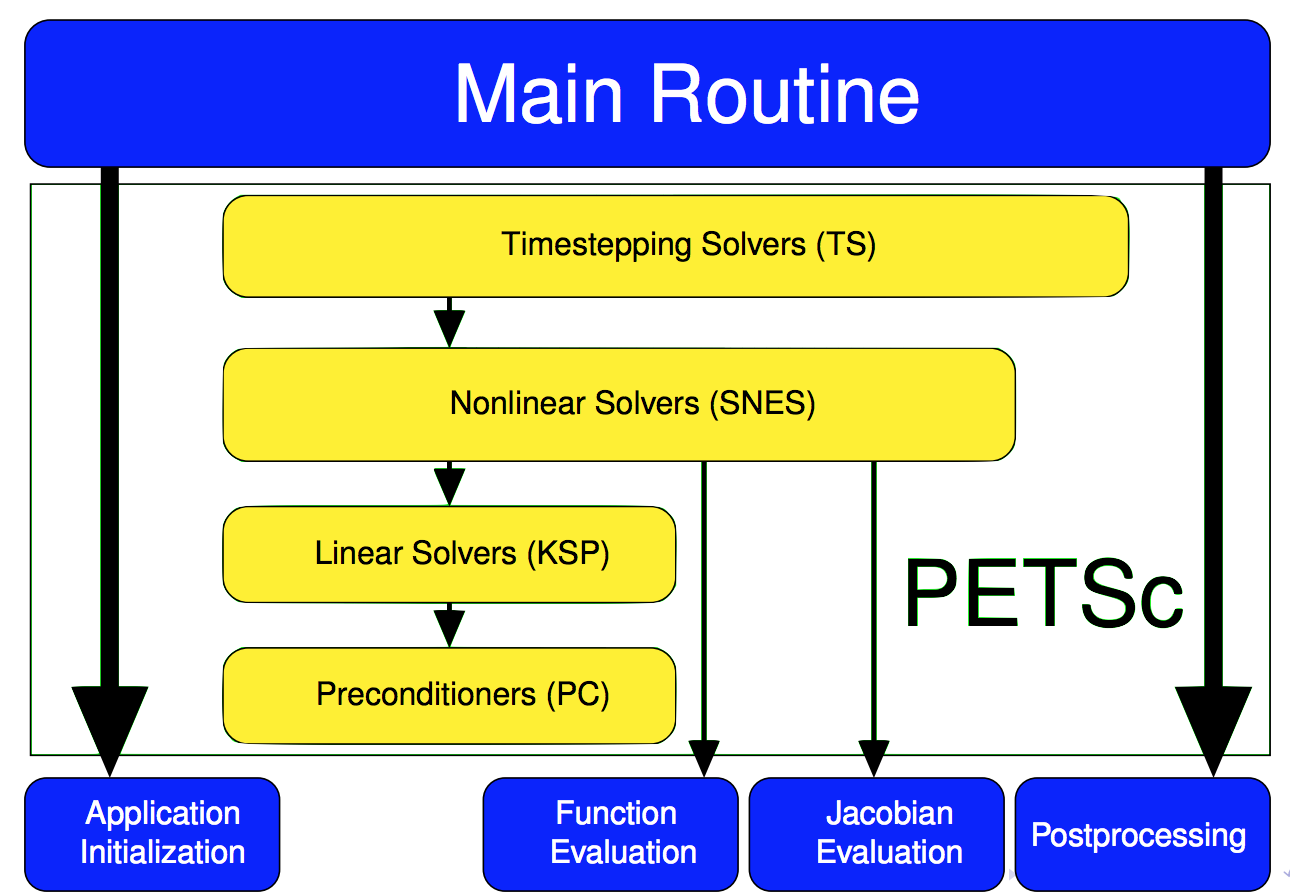
\includegraphics[width=0.7\linewidth]{figures/FlowControlForPETScApplication.png}
\end{center}
\caption{Flow control for a PETSc application. [Source: PETSc tutorial https://www.mcs.anl.gov/petsc/documentation/tutorials]\label{fig:petscFlow}}
\end{figure}

%PETSc
This dissertation focuses on using solvers and preconditioners offered by PETSc~\cite{petsc}. Portable Extensible Toolkit for Scientific Computing (PETSc) is a widely used toolkit for linear systems, developed at Argonne National Laboratory. PETSc is a collection of data structures and functions for the scalable (parallel) solution of scientific applications and offers solver techniques and preconditioners for linear and non-linear equations. PETSc can run on different architectures, various operating systems and is portable to any parallel system that supports MPI. PETSc is widely used for modeling small-scale and large-scale applications and is considered to be a highly efficient toolkit. PETSc offers scalable solutions for scientific applications ranging from brain surgery~\cite{petscapp1}, cancer treatment~\cite{petscapp2}, earthquakes~\cite{petscapp3}, ocean dynamics~\cite{petscapp4}, among many others. Figure~\ref{fig:petscFlow} shows the flow control for a PETSc application. The rest of the section describes some of the most popular Krylov subspace methods for symmetric and non-symmetric matrices offered by PETSc and used throughout this research. 

% \subsection{ Jacobi Method}
% Jacobi method is a solver technique in which the original matrix $A$ is split into matrices, say, $D$ and $T$, such that, $A = D - (L + U)$, where $D$ is the diagonal of the matrix $A$, $L$ is the strict lower part of the original matrix $A$ and $U$ is the strict upper part of the matrix $A$. The decomposition can be shows as below: 
% \begin{center}
% $D = diag(A)$, and $A = D - L - U$
% \end{center}

% Once the matrix is decomposed into the diagonal, lower and upper triangular, the transformed systems can be shown as below:
% \begin{center}
% $Ax = b$ and $A = D - L - U$, where $D = diag(A)$

% $(D - L - U)x = b$ \\
% For each iteration, the next successive solution is obtained by applying the following rule:
% $x_{(k+1)} = D^{-1}(E+F)x_{k} + D^{-1} b$
% \end{center}

% As the number of iteration progress, the asolution approximation is expected to improve.
% This is a solver method that is common for diagonally dominant system. One of the reasons it is very popular is because it is highly parallelizable.

\subsection{Conjugate Gradient Method and variants of Conjugate Gradient}

Conjugate Gradient (CG) method ~\cite{cg1,cg2,cg3} is applicable for symmetric linear systems. CG starts with an initial guess of the
solution, an initial residual and an initial search direction. It looks for approximate solutions at each step within its Krylov subspace as shown below: 
\begin{center}
${K}_{k} = span\{b,Ab,A^{2}b,\ldots,A^{k-1}b\}$ for $k \geq 1$
\end{center}
It finds a series of gradients (conjugate vectors) $x^{0}, x^{1}, \ldots$ until the point where the gradient gets sufficiently close to the solution. The gradients are given by the equation shown below: 
\begin{center}
$x_{k+1} = x_{k} + \alpha_k s_k$
\end{center}  
Here $\alpha_k$ is a scalar determining the step length and $ s_k$ is the search direction. The minimum over $\alpha $ occurs when the residual is orthogonal to the search direction. Each iteration requires only one matrix-vector multiplication. They are also the gradients of a quadratic function shown below, the minimization of which is the same as solving the system:
\begin{center}
$\phi(x) = 1/2 x^{T}Ax - x^{T} b $.
\end{center}
Initially, $s_0 = r_0 = b - ax_0$, and the residual is updated in the following way:
\begin{center}
$r_{k+1} = b - Ax_{k+1} = r_k - \alpha_k A s_k$.
\end{center}
The storage requirement of Conjugate Gradient is low, as it only needs to store vectors $x$, $r$ and $s$, and they can be overwritten after each iteration. The convergence rate depends on the square root of the condition number. It is an extremely popular solver technique for symmetric, positive definite matrices. Conjugate Gradient method became the ground for many other solver methods, which were variants of Conjugate Gradient, such as BiConjugate Gradient method, BiConjugate Gradient Stabilized method, Conjugate Gradient Squared and Improved Stabilized version of BiConjugate Gradient Squared method (some of which are described in the following section).



\subsection{Chebyshev Method}
\subsection{QMR Method}
\subsection{GMRES Method}
\subsection{LSQR Method}
\subsection{Jacobi Method}
\subsection{Gauss-Seidel Method}
\subsection{SOR Method}


\section{Single-Method Solver Systems}

\section{Multi-Method Solver Systems}
\subsection{Composite Solver System}
\subsection{Adaptive Solver System}
\subsection{Poly-iterative Solver System}
\subsection{SALSA System}
\subsection{LSA Solver System}
\subsection{FETI}


\section{Summary}